\documentclass[12pt,a4paper]{report}
\usepackage[utf8]{vietnam}\usepackage{amsmath, amsthm, amssymb,latexsym,amscd,amsfonts,enumerate}
\usepackage[top=3.5cm, bottom=3.0cm, left=3cm, right=3.0cm]{geometry} 
\usepackage{color, fancyhdr, graphicx, wrapfig}
\usepackage[unicode]{hyperref}
\usepackage[vietnamese]{babel}
\usepackage{titling}
\usepackage{subfigure}
\usepackage{secdot}
\usepackage{enumitem}
\usepackage{array}
\usepackage[tikz]{ocgx2}
\usepackage{xcolor}
\usepackage{blindtext}
\usepackage{multicol}
\usepackage{tikz}
\usepackage{subcaption}
\usepackage{changepage}
\usepackage{float}
\usepackage{pgfplotstable}
\usepackage{pgfplots}
\usepackage{blindtext}
\usepackage{titlesec}
\usepackage{mathtools}
\usepackage{tabularx}
\usepackage{nccmath}
\usetikzlibrary{calc}
\usepackage{longtable}
\usepackage{indentfirst}
\usepackage{fancyhdr}
\usepackage{exscale,relsize,makeidx}
%\usepackage{refcheck}
\setcounter{tocdepth}{4}
\setcounter{secnumdepth}{4}
\newtheorem{dn}{Định nghĩa}
\newtheorem{tc}{Tính chất}
\newtheorem{dl}{Định lý}
\newtheorem{md}{Mệnh đề}
\newtheorem{bd}{Bổ đề}
\newtheorem{hq}{Hệ quả}
\newtheorem{nx}{Nhận xét}
\newtheorem{vd}{Ví dụ}
\newtheorem{cy}{Chú ý}
\pagenumbering{roman}\pagestyle{plain}
%\pagestyle{fancy}
%\lhead{\it \changefontsizes{11pt}Luận văn thạc sĩ:}
%\rhead{\it Một số phương pháp vô hướng hóa cơ bản trong tối ưu đa mục tiêu}
%\lfoot{\it Nguyễn Văn Vân } 			         
%\rfoot{\it K19.2 trường ĐHSG}
\renewcommand{\headrulewidth}{1,2pt} 			
\renewcommand{\footrulewidth}{1,2pt}
\newcommand{\dstc}[2]
{
	\newdimen\stringwidth\setbox0=\hbox{#1}
	\stringwidth=\wd0
	\hspace*{-\parindent}\hspace*{.5\textwidth}\hspace*{-.5\wd0}#1\hfill #2\bigskip
	
}  
\usepackage{scrextend}
\fancyhf{}
\lhead{}
\chead{\thepage}
\rhead{}
\cfoot{}
\rfoot{}
\lfoot{}
\pagestyle{fancy}
\renewcommand{\headrulewidth}{1pt}
\begin{document} 
\subsection{Phương pháp hình học}
\subsubsection*{Vấn đề về tập lồi}
\usetikzlibrary{patterns}

\begin{dn}[Tập lồi]
Tập $S$ được gọi là \textbf{tập lồi} nếu $S$ thoả điều kiện:
\begin{itemize}
\item Cho bất kỳ 2 điểm $A$ và $B$ nằm trong tập $S$.
\item Đường thẳng nối 2 điểm $A$ và $B$ luôn nằm trong $S$.
\end{itemize}
\end{dn}


\begin{dn}[Cực điểm]
Với bất kỳ tập $S$, điểm $P \in S$ được gọi là \textbf{cực điểm} nếu thoả các điều kiện:
\begin{itemize}
\item Tồn tại đoạn thẳng $AB$ nằm hoàn toàn trong $S$.
\item Tồn tại điểm $P$ sao cho $P := \{x \in AB: x=A \vee x=B \}$.
\end{itemize}
\end{dn}

\begin{dn}[Siêu phẳng]
Tập $S$ gọi là một \textbf{siêu phẳng} nếu $S$ gồm các vector
\begin{equation*}
X = \begin{bmatrix}
        x_1 \\
        x_2 \\
        \vdots \\
        x_n
	\end{bmatrix}
\end{equation*}
trong không gian $\mathbb{R}^n$ sao cho
\begin{equation*}
a_1x_1 + a_2x_2 + \ldots + a_nx_n = c
\end{equation*}
trong đó $c$ là một hằng số và $a_1,a_2,\ldots,a_n \neq 0$.
\end{dn}
\begin{figure}
	\centering
	\subfigure[]{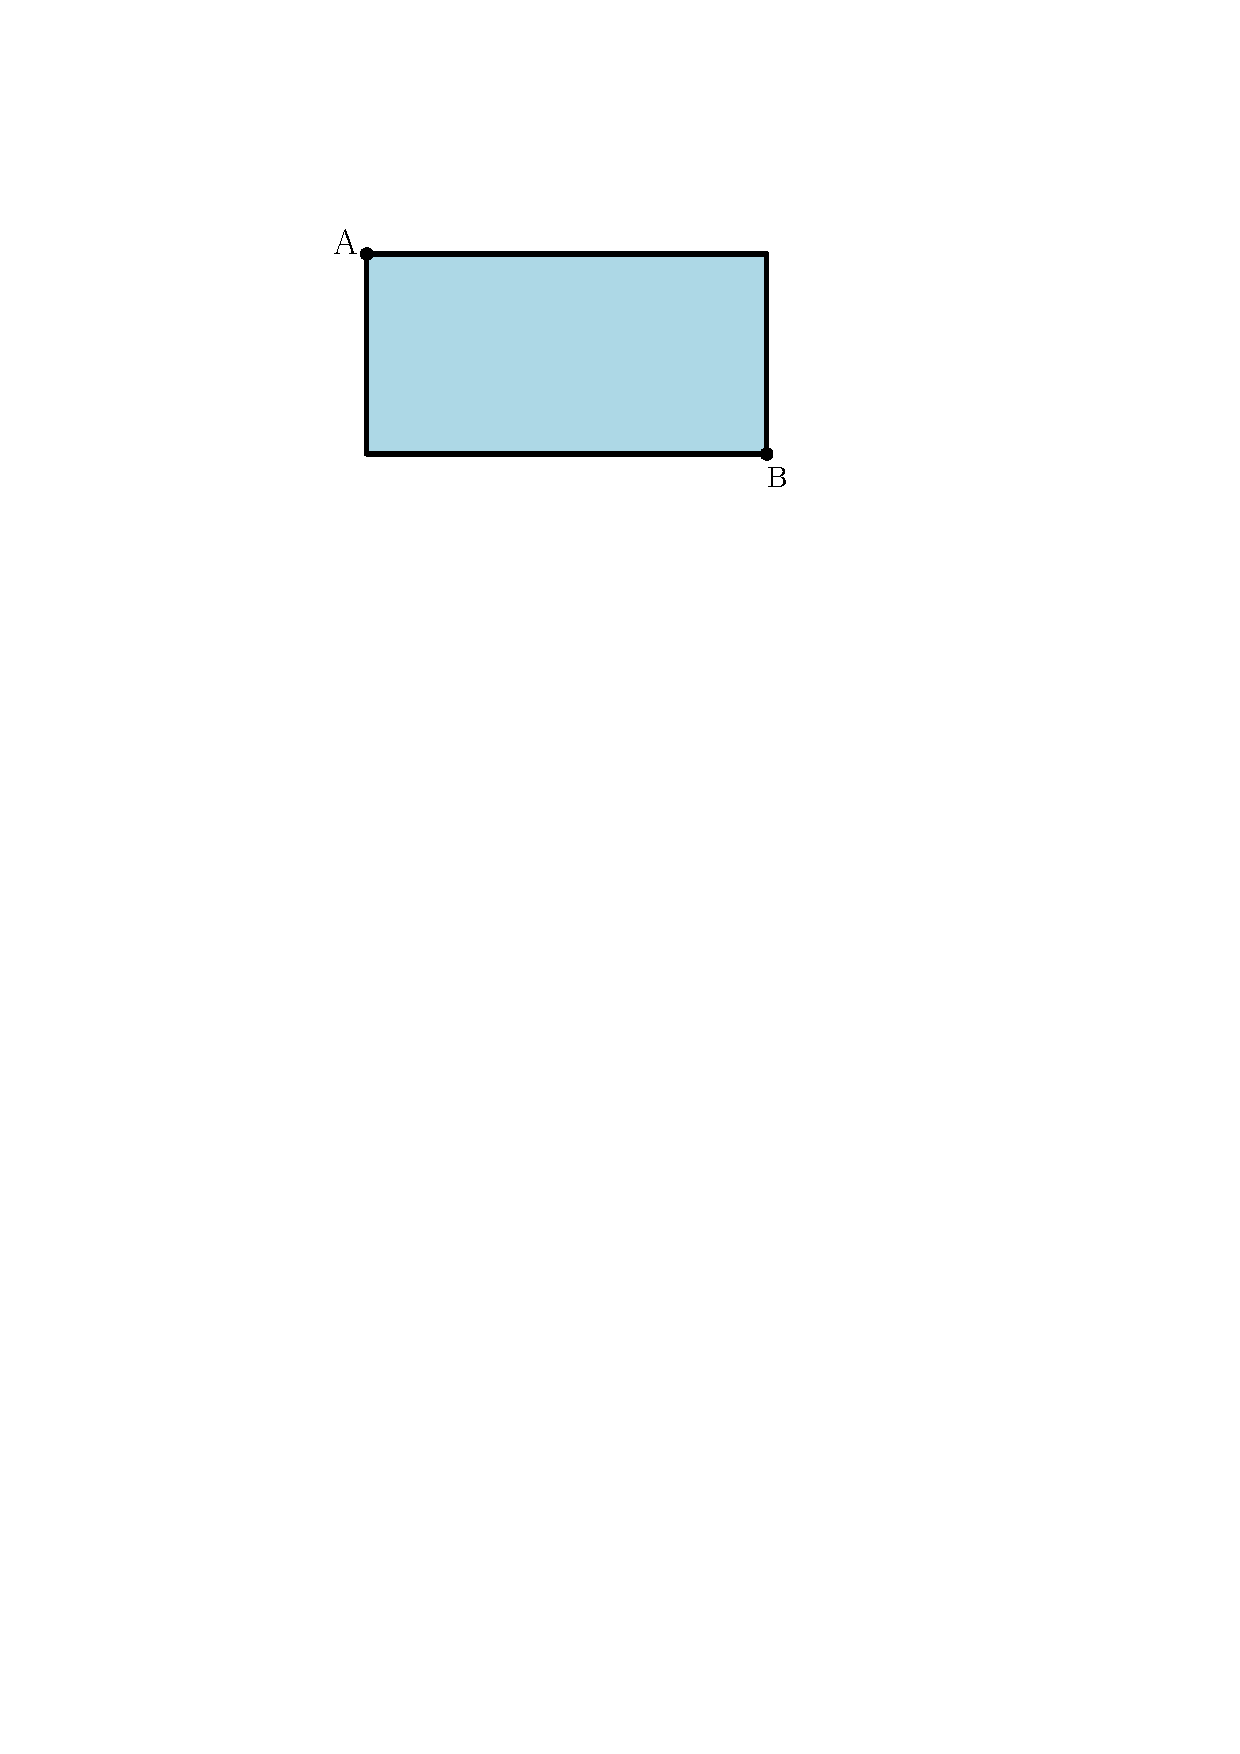
\includegraphics[width=0.2\textwidth]{vuong2.pdf}} 
	\subfigure[]{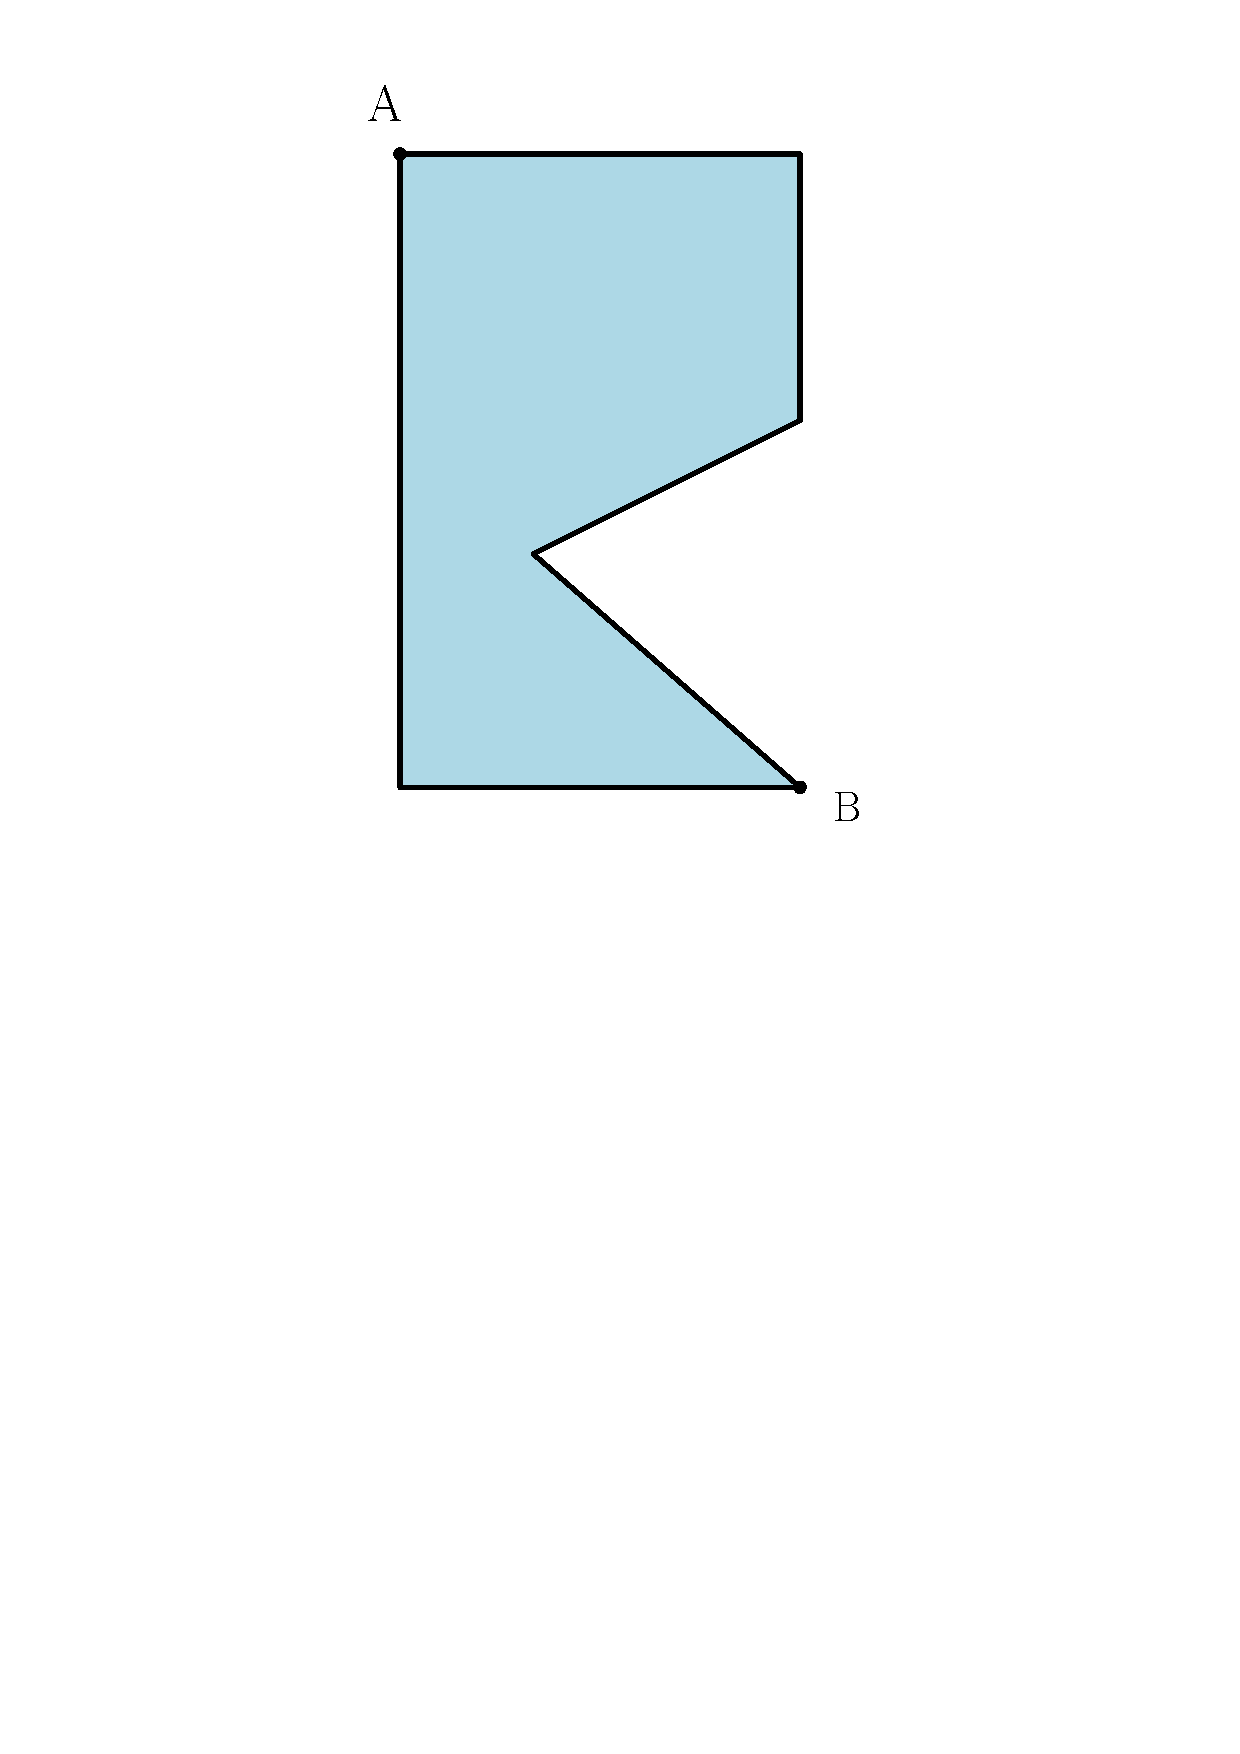
\includegraphics[width=0.15\textwidth]{lom.pdf}} 
	\subfigure[]{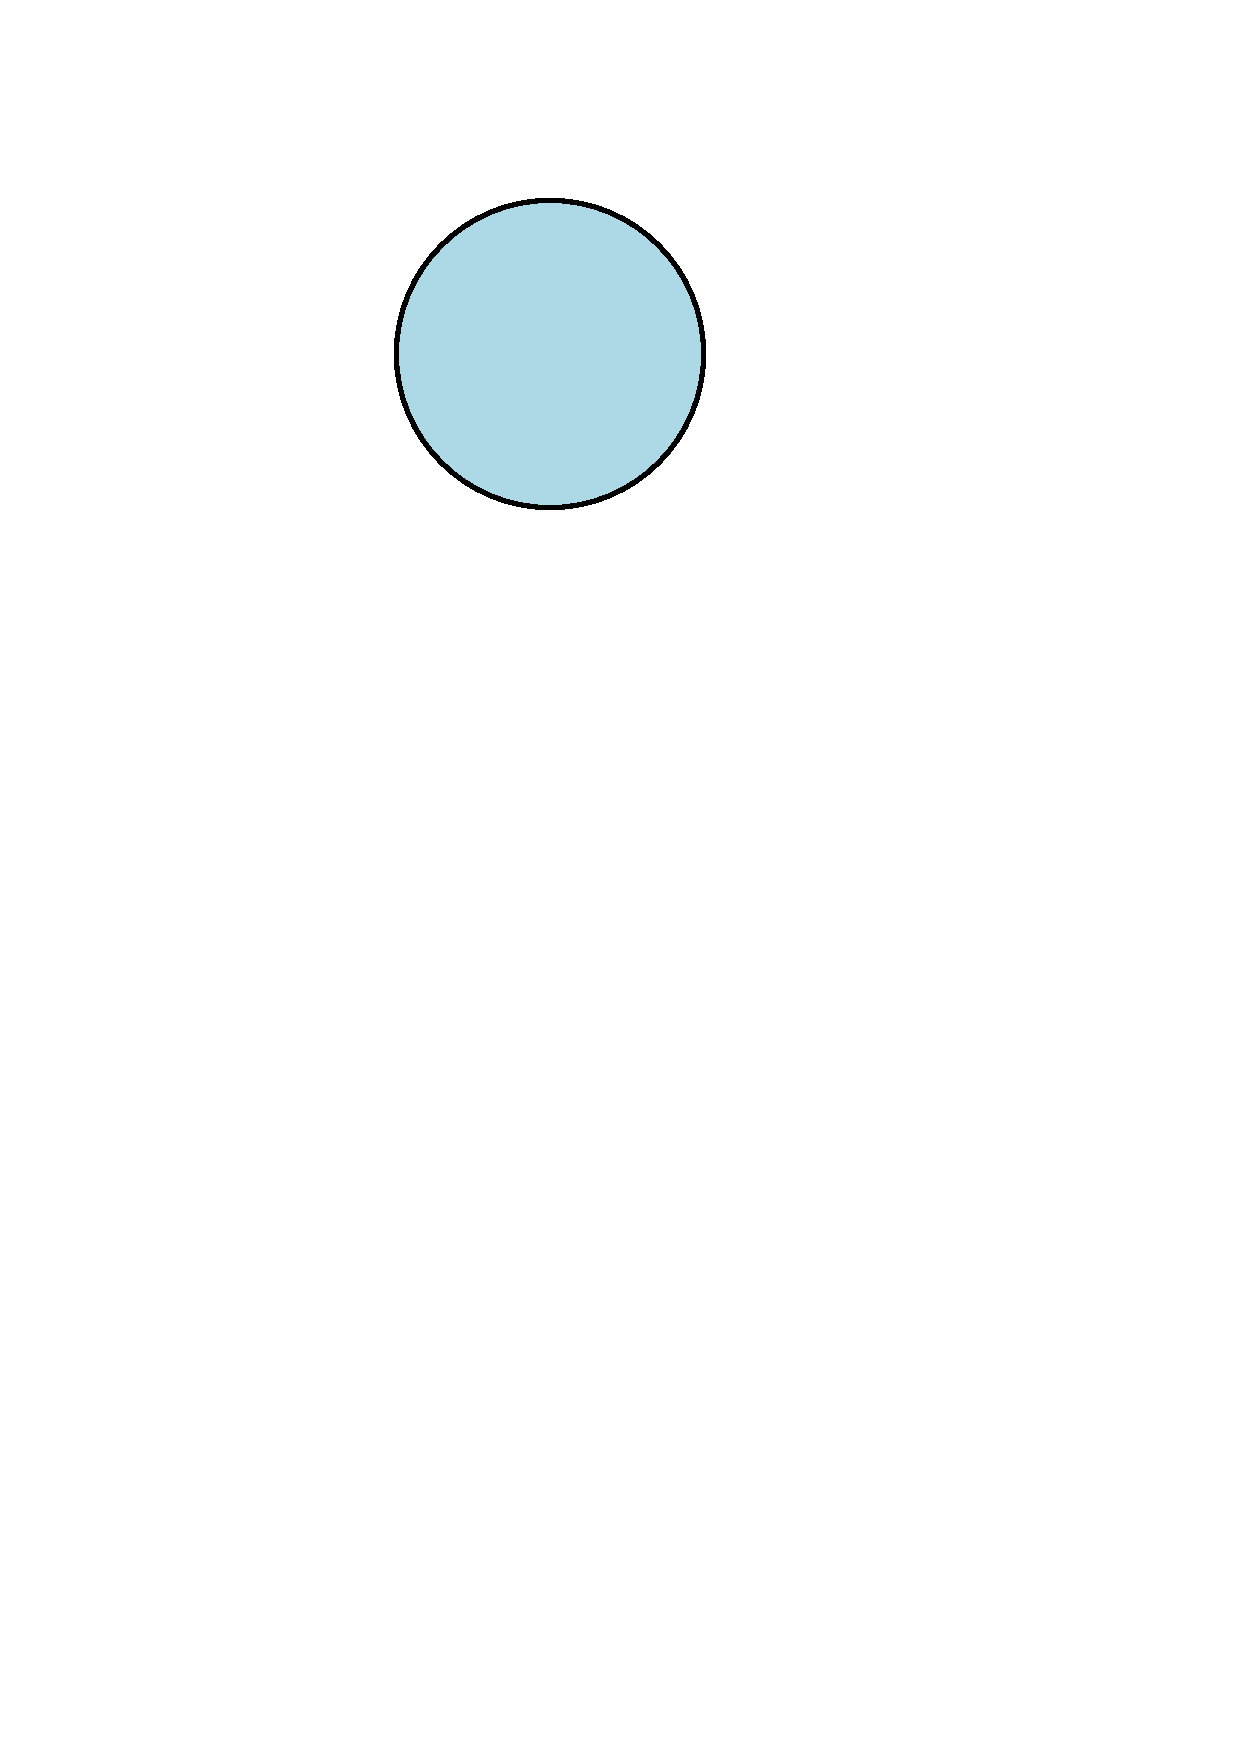
\includegraphics[width=0.15\textwidth]{tron.pdf}} 
	\subfigure[]{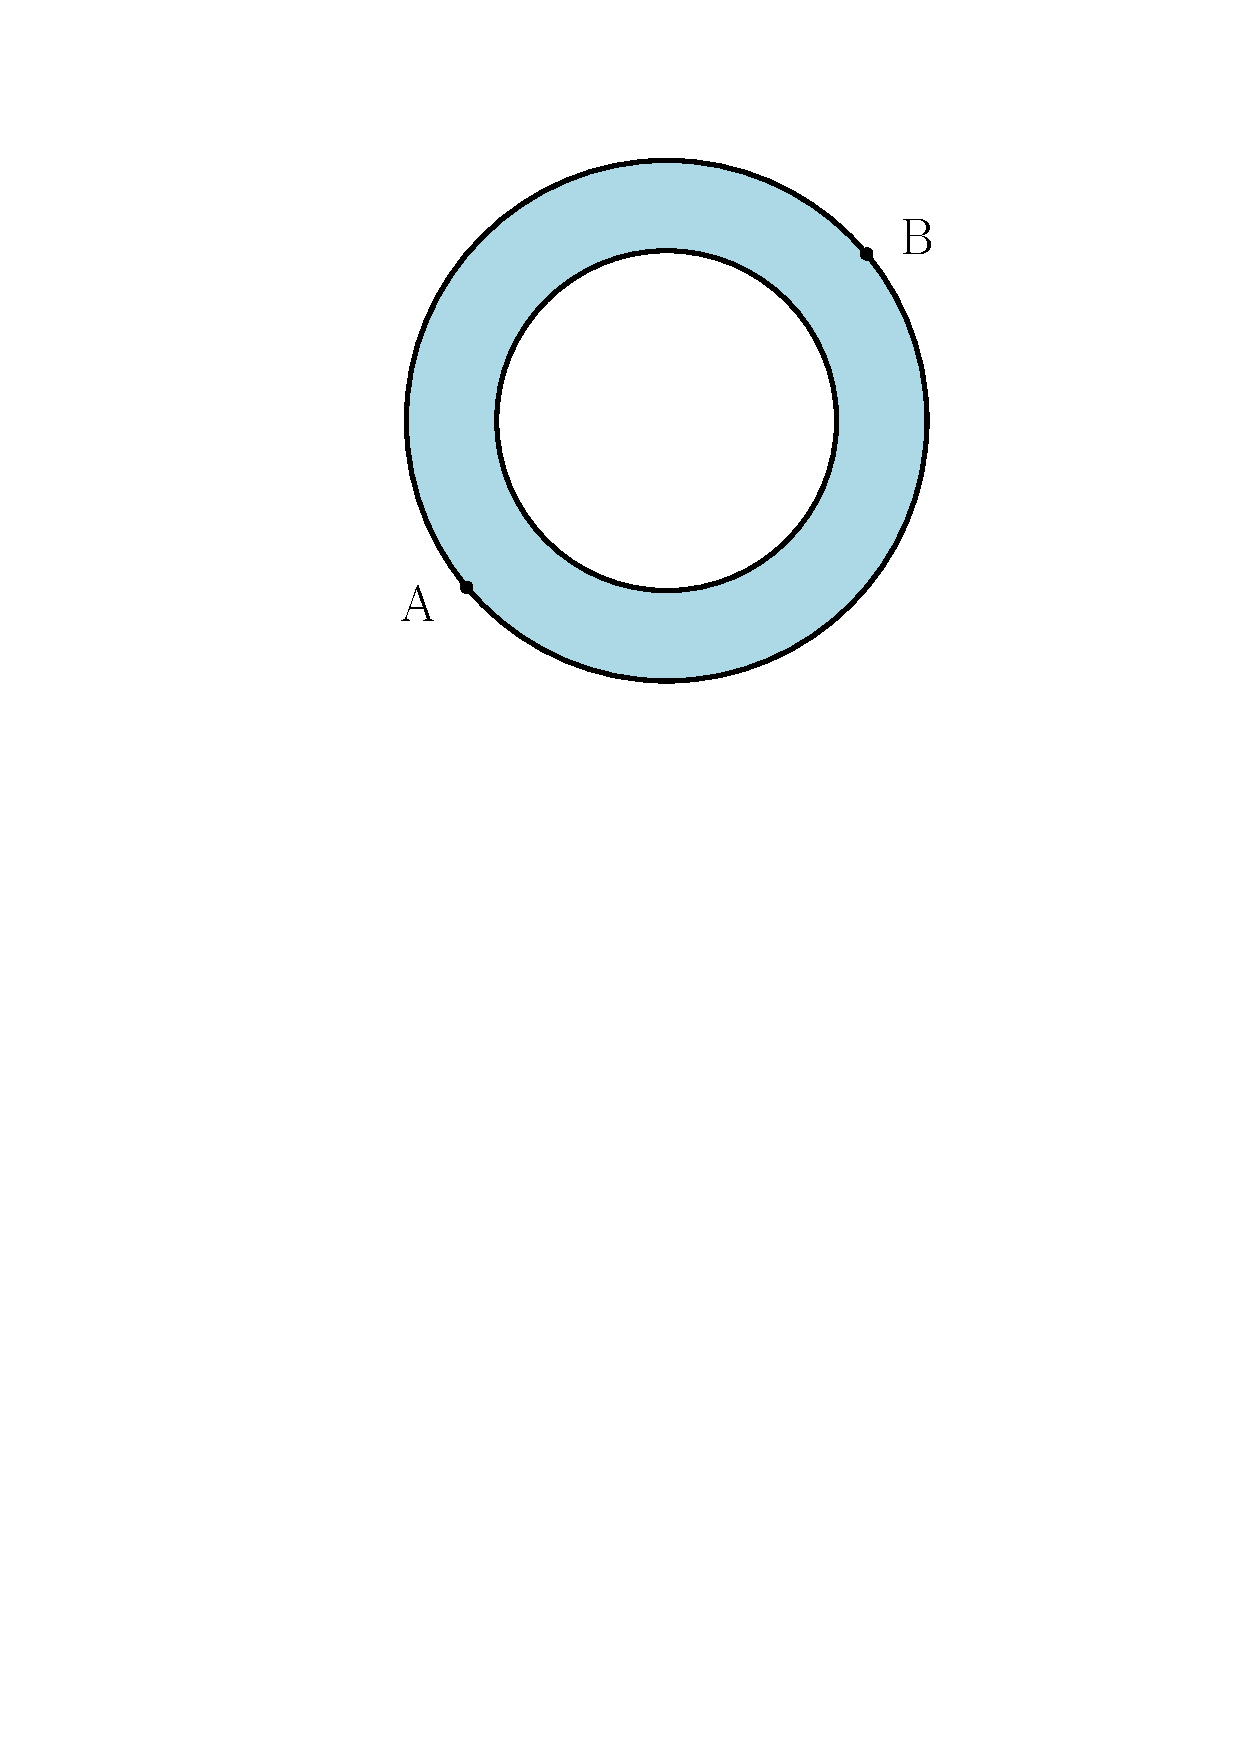
\includegraphics[width=0.15\textwidth]{duc lo.pdf}} 
	\caption{(a) Tập lồi (b) Tập lõm (c) Tập lồi (d) Tập lõm}
	\label{fig:foobar}
\end{figure}

\subsubsection*{Bài toán trong không gian $\mathbb{R}^2$}

\begin{equation} \small \label{chinhtac}
	\begin{split}
	(P) \quad \text{Min } & f(x) = c^Tx \\
		& \left\{
		\begin{split}
		& Ax=b, \\
		& x_j \geq 0, \:\: j=1,2.
		\end{split}
		\right.    
	\end{split}
\end{equation}
Trong đó $A$ là ma trận $m\times 2$, $b=\begin{pmatrix}
	b_1 \\
	b_2 \\
	\vdots \\
	b_m
	\end{pmatrix}$ và $c^T=(c_1 \: c_2 )$.


\begin{itemize}
\item \textbf{Tập nghiệm của bài toán}

Ta có bài toán minh hoạ sau:
\begin{equation}
	\begin{split}
	(P) \quad & f(x) = 3x_1 + 2x_2 \longrightarrow Max \\
		& \left\{\begin{split}
		x_1 + x_2 &\leq 7 \\
		2x_1 + x_2 &\leq 10 \\
		x_1 &\leq 4 \\
		x_1, x_2 &\geq 0. \\
		\end{split}\right.    
	\end{split}
\end{equation}
Với từng ràng buộc, ta có thể biểu thị trên đồ thị bằng từng đường thẳng tương ứng, ví dụ, ràng buộc
\begin{equation*}
x_1 + x_2 \leq 7
\end{equation*}
tương ứng với mặt phẳng bên dưới đường thẳng $CD$ trong hình 2.
\begin{equation*}
	2x_1 + x_2 \leq 10
\end{equation*}
tương ứng với mặt phẳng bên dưới đường thẳng $AB$.
\begin{equation*}
	x_1 \leq 4
	\end{equation*}
tương ứng với mặt phẳng bên trái đường thẳng $EG$. Tập nghiệm của bài toán là đa giác $OCKGE$ được biểu thị trong đồ thị hình 2.

\item \textbf{Phương án tối ưu của bài toán}
\begin{itemize}
\item Để tìm phương án tối ưu của bài toán ta thiết lập phương thay đổi của hàm mục tiêu
\begin{equation*}
f(x)=c_1x_1+c_2x_2,
\end{equation*}
trong đó phương trình mô tả họ đường thẳng phụ thuộc theo tham số $f(x)$ với pháp vector $v=(c_1,c_2)$, giá trị $f(x)$ tăng hoặc giảm theo một hướng của vector v.
\item Từ phương trình hàm mục tiêu ta thiết lập các đường mức.
\item Tịnh tiến song song các đường mức theo chiều tăng nếu Max hoặc giảm nếu Min để tìm phương án tối ưu của bài toán. (Hình 3)
\end{itemize}

\begin{figure}[!htb]\label{hinh2}
    \begin{minipage}{0.48\textwidth}
            \center
            \begin{tikzpicture}
            \begin{axis}
                [
                xmin=0,xmax=10,
                ymin=0,ymax=15,
                xlabel={$x_1$},
                ylabel={$x_2$},
                grid style={line width=.1pt, draw=darkgray!50},
                major grid style={line width=.2pt,draw=darkgray!50},
                axis lines=middle,
                yticklabel=\empty,
                xticklabel=\empty,
                enlargelimits={abs=0},
                samples=10,
                domain = 0:1,
                ]
                \filldraw[blue!50, pattern=north west lines, pattern color=blue!90, line width=1.5pt] (0, 0) -- (0, 70) -- (30, 40) -- (40, 20) -- (40, 0) -- cycle;
                \draw (0, 70) -- (70, 0);
                \draw (0, 100) -- (50, 0);
                \draw (40, 0) -- (40, 90);
                \node at (3, 4) {\tiny O};
                \node at (4, 72) {\tiny C};
                \node at (42, 4) {\tiny E};
                \node at (43, 20) {\tiny G};
                \node at (32, 43) {\tiny K};
                \node at (72, 4) {\tiny D};
                \node at (52, 4) {\tiny B};
                \node at (5, 100) {\tiny A};
                \node at (0, 100) {\tiny \textbullet};
                \node at (0, 70) {\tiny \textbullet};
                \node at (30, 40) {\tiny \textbullet};
                \node at (40, 20) {\tiny \textbullet};
                \node at (40, 0) {\tiny \textbullet};
                \node at (50, 0) {\tiny \textbullet};
                \node at (70, 0) {\tiny \textbullet};
                \node at (0, 0) {\tiny \textbullet};
            \end{axis}
            \end{tikzpicture}  
            \caption{Đa giác $OCKGE$ là tập nghiệm của bài toán (P).}
    \end{minipage}\hfill
    \begin{minipage}{0.48\textwidth}
            \center
            \begin{tikzpicture}
            \begin{axis}
                [
                xmin=0,xmax=10,
                ymin=0,ymax=15,
                xlabel={$x_1$},
                ylabel={$x_2$},
                grid style={line width=.1pt, draw=darkgray!50},
                major grid style={line width=.2pt,draw=darkgray!50},
                axis lines=middle,
                yticklabel=\empty,
                xticklabel=\empty,
                enlargelimits={abs=0},
                samples=10,
                domain = 0:1,
                ]
                \filldraw[blue!30, pattern=north west lines, pattern color=blue!30, line width=1pt] (0, 0) -- (0, 70) -- (30, 40) -- (40, 20) -- (40, 0) -- cycle;
                \draw (0, 70) -- (70, 0);
                \draw (0, 100) -- (50, 0);
                \draw (40, 0) -- (40, 90);
                \draw[dotted, line width = 1.5pt] (0, 80) -- (60, 0);
                \draw[->, line width = 1.5pt] (0, 0) -- (15, 20);
                \node at (3, 4) {\tiny O};
                \node at (4, 72) {\tiny C};
                \node at (42, 4) {\tiny E};
                \node at (43, 20) {\tiny G};
                \node at (34, 45) {\small \textbf{K}};
                \node at (72, 4) {\tiny D};
                \node at (52, 4) {\tiny B};
                \node at (5, 100) {\tiny A};
                \node at (0, 100) {\tiny \textbullet};
                \node at (0, 70) {\tiny \textbullet};
                \node at (30, 40) {\small \textbullet};
                \node at (40, 20) {\tiny \textbullet};
                \node at (40, 0) {\tiny \textbullet};
                \node at (50, 0) {\tiny \textbullet};
                \node at (70, 0) {\tiny \textbullet};
                \node at (0, 0) {\tiny \textbullet};
            \end{axis}
            \end{tikzpicture}  
            \caption{Minh hoạ phương pháp tìm phương án tối ưu của bài toán (P).}
    \end{minipage}
 \end{figure}

\end{itemize}

\subsubsection*{Các trường hợp đặc biệt}
\begin{itemize}
\item \textbf{Vô nghiệm}

Trường hợp bài toán có các ràng buộc không cùng tạo ra miền nghiệm của bài toán, xem Hình 4. thì bài toán được gọi là vô nghiệm.
\item \textbf{Vô số nghiệm}

Trường hợp bài toán có đường mức được tạo ra từ phương trình hàm mục tiêu song song với cực biên của tập nghiệm, bài toán cho ra vô số nghiệm. (Hình 5)
\begin{figure}[!htb]
    \begin{minipage}{0.48\textwidth}
    \center
    \begin{tikzpicture}
    \begin{axis}
        [
        xmin=0,xmax=10,
        ymin=0,ymax=15,
        xlabel={$x_1$},
        ylabel={$x_2$},
        grid style={line width=.1pt, draw=darkgray!50},
        major grid style={line width=.2pt,draw=darkgray!50},
        axis lines=middle,
        yticklabel=\empty,
        xticklabel=\empty,
        enlargelimits={abs=0},
        samples=10,
        domain = 0:1,
        ]
        \draw (0, 70) -- (70, 0);
        \draw (0, 100) -- (50, 0);
        \draw (60, 0) -- (60, 90);
        \draw (0, 40) -- (80, 40);
        \node at (3, 4) {\tiny O};
        \node at (4, 72) {\tiny C};
        \node at (32, 45) {\tiny K};
        \node at (72, 4) {\tiny D};
        \node at (52, 4) {\tiny B};
        \node at (5, 100) {\tiny A};
        \node at (0, 100) {\tiny \textbullet};
        \node at (0, 70) {\tiny \textbullet};
        \node at (30, 40) {\tiny \textbullet};
        \node at (50, 0) {\tiny \textbullet};
        \node at (70, 0) {\tiny \textbullet};
        \node at (0, 0) {\tiny \textbullet};
    \end{axis}
    \end{tikzpicture}  
    \caption{Minh hoạ trường hợp bài toán vô nghiệm.}
    \end{minipage}\hfill
    \begin{minipage}{0.48\textwidth}
    \center
    \begin{tikzpicture}
    \begin{axis}
        [
        xmin=0,xmax=10,
        ymin=0,ymax=15,
        xlabel={$x_1$},
        ylabel={$x_2$},
        grid style={line width=.1pt, draw=darkgray!50},
        major grid style={line width=.2pt,draw=darkgray!50},
        axis lines=middle,
        yticklabel=\empty,
        xticklabel=\empty,
        enlargelimits={abs=0},
        samples=10,
        domain = 0:1,
        ]
        \filldraw[blue!30, pattern=north west lines, pattern color=blue!30, line width=1pt] (0, 0) -- (0, 70) -- (30, 40) -- (40, 20) -- (40, 0) -- cycle;
        \draw (0, 70) -- (70, 0);
        \draw (0, 100) -- (50, 0);
        \draw (40, 0) -- (40, 90);
        \draw[dotted, line width=2pt] (0, 25.94) -- (13, 0);
        \draw[->] (0, 0) -- (20, 30);
        \node at (3, 4) {\tiny O};
        \node at (4, 72) {\tiny C};
        \node at (42, 4) {\tiny E};
        \node at (43, 20) {\tiny G};
        \node at (32, 43) {\tiny K};
        \node at (72, 4) {\tiny D};
        \node at (52, 4) {\tiny B};
        \node at (5, 100) {\tiny A};
        \node at (0, 100) {\tiny \textbullet};
        \node at (0, 70) {\tiny \textbullet};
        \node at (30, 40) {\tiny \textbullet};
        \node at (40, 20) {\tiny \textbullet};
        \node at (40, 0) {\tiny \textbullet};
        \node at (50, 0) {\tiny \textbullet};
        \node at (70, 0) {\tiny \textbullet};
        \node at (0, 0) {\tiny \textbullet};
    \end{axis}
    \end{tikzpicture}  
    \caption{Minh hoạ trường hợp bài toán có vô số nghiệm.}
    \end{minipage}
\end{figure}
\item \textbf{Giá trị tối ưu đạt vô hạn}

Trường hợp miền nghiệm của bài toán là một tập mở đồng thời pháp vector cho chiều vô hạn thì bài toán có giá trị tối ưu đạt vô cực. (Hình 6)
\begin{figure}
    \center
    \begin{tikzpicture}
    \begin{axis}
        [
        xmin=0,xmax=10,
        ymin=0,ymax=15,
        xlabel={$x_1$},
        ylabel={$x_2$},
        grid style={line width=.1pt, draw=darkgray!50},
        major grid style={line width=.2pt,draw=darkgray!50},
        axis lines=middle,
        yticklabel=\empty,
        xticklabel=\empty,
        enlargelimits={abs=0},
        samples=10,
        domain = 0:1,
        ]
        \filldraw[blue!30, pattern=north west lines, pattern color=blue!30, line width=1pt] (0, 200) -- (0, 40) -- (22, 10.5) -- (220, 180) -- cycle;

        \draw (0, 40) -- (30, 0);
        \draw (10, 0) -- (80, 60);
        \draw[->] (0, 0) -- (10, 20);
        \node at (4, 44) {\tiny O};
        \node at (33, 6) {\tiny C};
        \node at (10, 6) {\tiny E};
        \node at (22, 16) {\tiny G};

        \node at (0, 40) {\tiny \textbullet};
        \node at (30, 0) {\tiny \textbullet};
        \node at (10, 0) {\tiny \textbullet};
        \node at (22, 10) {\tiny \textbullet};
    \end{axis}
    \end{tikzpicture}  
    \caption{Minh hoạ trường hợp bài toán có giá trị vô hạn.}
\end{figure}
\end{itemize}
\end{document}